\documentclass[conference]{IEEEtran}
\IEEEoverridecommandlockouts

% pdfLaTeX (e.g. Overleaf) uses IEEEtran's Times; XeTeX/Tectonic needs the Times clone set explicitly.
\usepackage{iftex}
\ifXeTeX
  \usepackage{fontspec}
  \setmainfont{texgyretermes}[Extension=.otf, UprightFont=*-regular, BoldFont=*-bold,
                              ItalicFont=*-italic, BoldItalicFont=*-bolditalic]
\fi

\usepackage{cite}
\usepackage{amsmath,amssymb}
\usepackage{graphicx}
\usepackage{booktabs}
\usepackage{multirow}
\usepackage{url}
\usepackage{xcolor}

\graphicspath{{figures/}}

\begin{document}

\title{Automatic Clothing Category Recognition on Fashion-MNIST: A Leakage-Controlled Comparison of Classical Models, Published CNNs and a Residual Network}

\author{\IEEEauthorblockN{Satyam Kumar, Krishna Verma, Akshit Vats, Chinmay Soni and Lakshya Bapna}
\IEEEauthorblockA{\textit{Department of Computer Science and Artificial Intelligence}\\
\textit{Newton School of Technology}\\
Project repository: \url{https://github.com/krishnaverma09/Fashion_Classifier_AML}}}

\maketitle

\begin{abstract}
Online retailers must assign a category to every product image, and doing so by hand is slow and inconsistent. We study automatic clothing category recognition on Fashion-MNIST, a ten-class benchmark of $28\times28$ grayscale images. Our study has three stages. First, Logistic Regression, $k$-nearest neighbours, Random Forest and a linear SVM are trained on raw pixels and on Histogram of Oriented Gradients (HOG) features under a shared 12,000-image budget. Second, a small convolutional neural network (CNN) is trained under the same budget. Third, we reimplement CNNs from three published studies and add a residual network (ResNet) with flip, shift and random-erasing augmentation, all trained on 48,000 images. Every model is selected on a fixed validation split, and each official test evaluation runs exactly once, after the choice has been frozen. The best classical model, Random Forest on pixels, reaches 85.27\% test accuracy and the small CNN 89.00\%. The ResNet reaches 94.32\%, and a three-model softmax ensemble chosen on validation reaches 94.19\%. The ResNet also has the smallest train--validation gap (2.0 points), and Shirt recall rises from 52.9\% to 82.1\%. The ResNet is deployed in a Gradio web demo with hash-verified weights.
\end{abstract}

\begin{IEEEkeywords}
image classification, Fashion-MNIST, convolutional neural networks, residual networks, data augmentation, HOG, random forest, overfitting
\end{IEEEkeywords}

\section{Introduction}
Clothing retailers manage catalogues with thousands of product photographs, and each one needs a category before it can be searched, filtered or recommended. Manual tagging is slow and tends to be inconsistent between annotators. Automatic category recognition is therefore a practical computer-vision problem, and Fashion-MNIST~\cite{xiao2017fashion} provides a standard benchmark for it. It was designed as a harder replacement for MNIST: its ten classes include visually similar upper-body garments (T-shirt/top, Pullover, Coat and Shirt) that remain difficult to separate at $28\times28$ resolution.

Many studies report Fashion-MNIST accuracies for classical models and CNNs~\cite{xiao2017fashion,kadam2020cnn,sumera2022cnn,edwards2019fashion,bhatnagar2017classification}. Their numbers are hard to compare, however, because training budgets, validation practice and test-set usage differ, and some studies leave them unspecified. This project compares all models under a single protocol. The training split, validation split and model choices are fixed before the test set is opened. The main contributions are:
\begin{itemize}
\item a budget-matched comparison of four classical classifiers on pixel and HOG features against a small CNN;
\item reimplementations of five networks from three published studies~\cite{sumera2022cnn,kadam2020cnn,edwards2019fashion}, trained and evaluated under one shared protocol;
\item a residual CNN with random-erasing augmentation that reaches 94.32\% test accuracy with the smallest train--validation gap of all networks;
\item a deployed Gradio~\cite{abid2019gradio} demo that serves the ResNet with hash-verified weights and a reproducible Docker setup.
\end{itemize}

\section{Related Work}
Xiao \textit{et al.}~\cite{xiao2017fashion} introduced Fashion-MNIST and benchmarked scikit-learn classifiers. An RBF-kernel SVC was the strongest at 89.7\%, ahead of Random Forest (87.3\%), $k$-NN (85.4\%) and Logistic Regression (84.2\%). Classical pipelines often replace raw pixels with HOG descriptors~\cite{dalal2005hog}, which summarise local edge orientations.

Sumera \textit{et al.}~\cite{sumera2022cnn} compared a dense ANN (784--3000--1000--10) with a two-layer CNN under SGD, Adagrad, RMSprop and Adam. The CNN trained with Adam was best, at 91\% test accuracy. Kadam \textit{et al.}~\cite{kadam2020cnn} evaluated five architectures and varied activation, optimizer, learning rate, dropout and batch size. Their Architecture~3 (three $2\times2$ convolutions) and Architecture~5 (VGG-style $3\times3$ convolutions) both reached 93.56\%. Edwards and Yen~\cite{edwards2019fashion} compared Bayesian discriminants, $k$-NN, decision trees and back-propagation networks with a Keras CNN. The CNN was best at 92.9\%, and classifier fusion did not improve on it.

Bhatnagar \textit{et al.}~\cite{bhatnagar2017classification} showed that batch normalisation~\cite{ioffe2015batch} and residual skip connections~\cite{he2016deep} raise a small CNN to 92.54\%. Zhong \textit{et al.}~\cite{zhong2017random} proposed random erasing, which occludes a random rectangle of each training image to reduce overfitting. Their wide residual networks reach error rates below 4\% on Fashion-MNIST. We build on these findings and evaluate them all under one protocol.

\section{Dataset and Evaluation Protocol}
\subsection{Fashion-MNIST}
Fashion-MNIST contains 70,000 grayscale images of $28\times28$ pixels in ten balanced classes: 60,000 official training images and 10,000 official test images (Fig.~\ref{fig:examples}). The archives are verified against the publisher's MD5 checksums. Pixels are scaled to $[0,1]$ and no other learned preprocessing is applied.

\begin{figure*}[t]
\centering
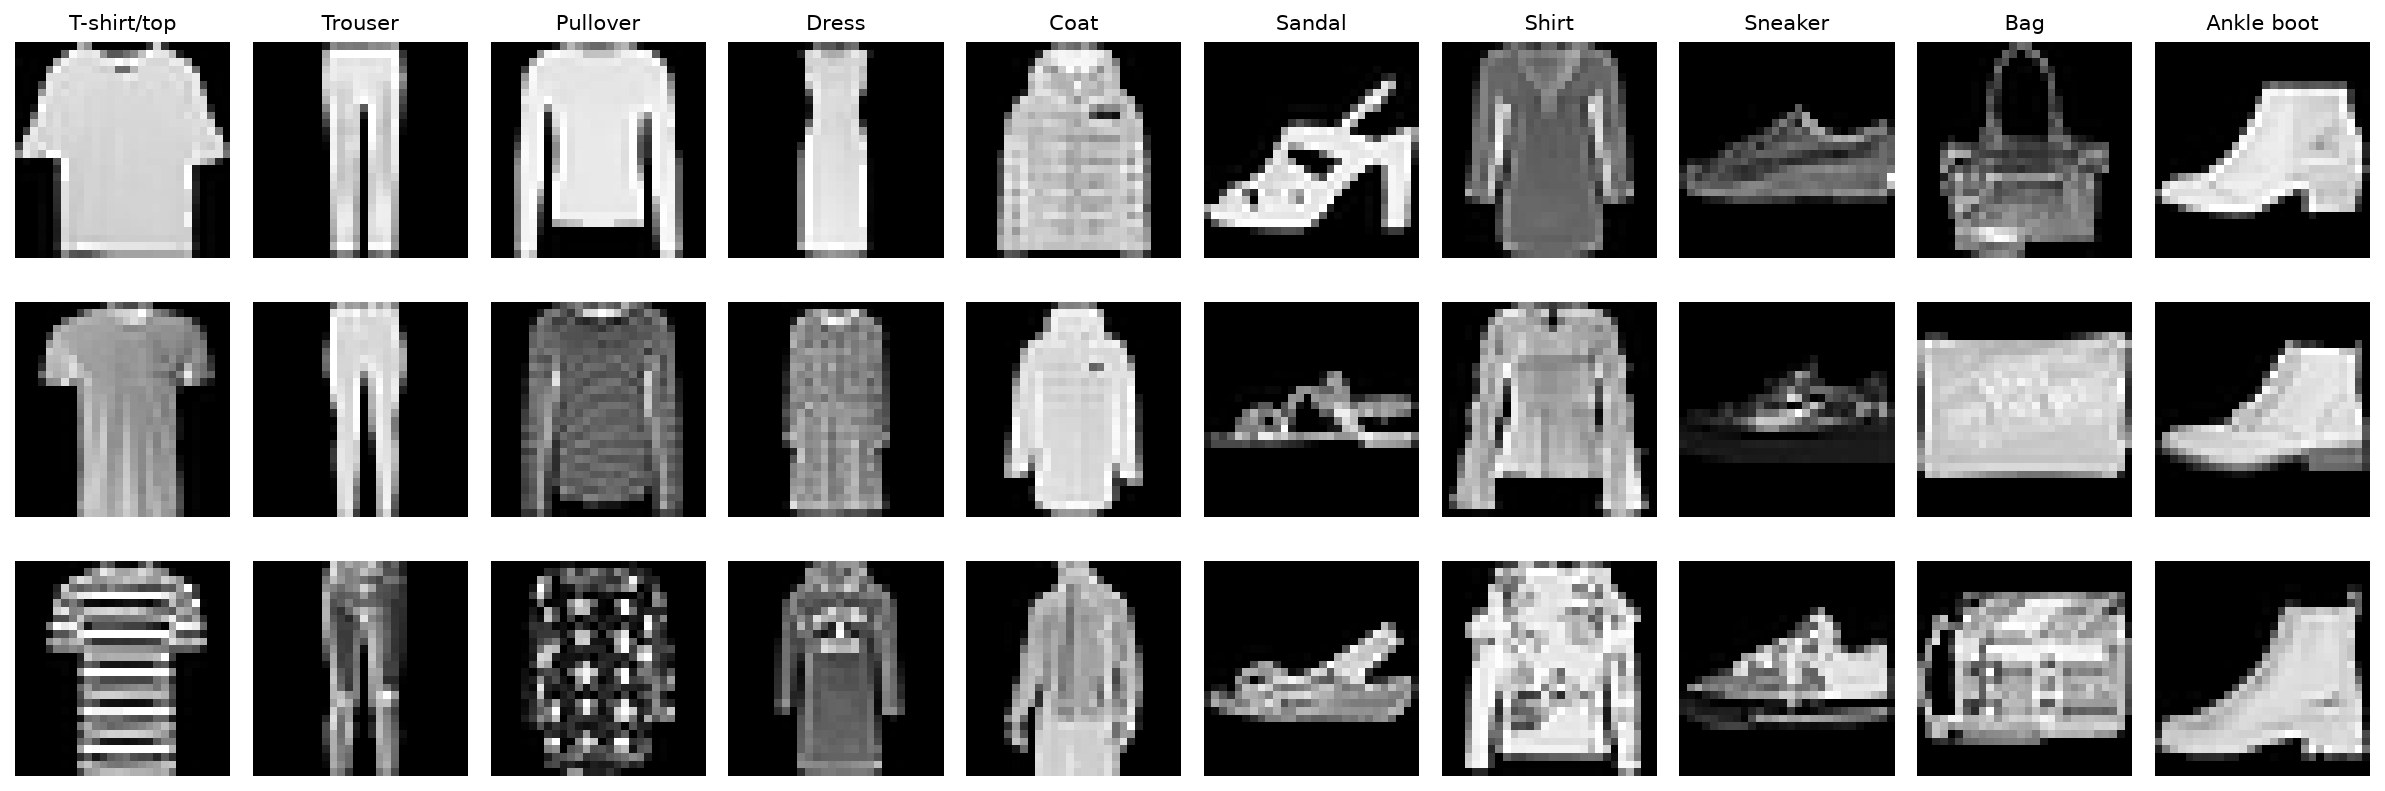
\includegraphics[width=0.92\textwidth]{dataset_examples.png}
\caption{Three training examples from each Fashion-MNIST class. Shirts share their outline with T-shirts, pullovers and coats, which is the main source of errors for every model.}
\label{fig:examples}
\end{figure*}

\subsection{Splits and Training Budgets}
A stratified split with seed 42 divides the official training images into 48,000 training and 12,000 validation images (4,800 and 1,200 per class). The split is saved with a fingerprint of the labels, and every experiment reloads it. The classical baselines and the small CNN share a saved 12,000-image subset of the training split (1,200 per class). The paper models and the ResNet use all 48,000 training images. Table~\ref{tab:splits} summarises the data.

\begin{table}[t]
\caption{Data splits used in this study}
\label{tab:splits}
\centering
\small
\begin{tabular}{@{}lrr@{}}
\toprule
Split & Images & Per class \\
\midrule
Training split (paper models, ResNet) & 48,000 & 4,800 \\
\quad Budget subset (baselines, small CNN) & 12,000 & 1,200 \\
Validation (selection, early stopping) & 12,000 & 1,200 \\
Official test (evaluated once) & 10,000 & 1,000 \\
\bottomrule
\end{tabular}
\end{table}

\subsection{Single-Use Test Protocol}
All model and hyperparameter choices use the validation split only. Before the official test set is opened, the chosen configurations and SHA-256 hashes of the model files are written to a frozen manifest. The test evaluation is then run once and never repeated for tuning, and further training is refused once the choice has been frozen. We report accuracy and macro-averaged $F_1$:
\begin{equation}
\mathrm{F_1^{macro}} = \frac{1}{10}\sum_{c=1}^{10}\frac{2\,P_c R_c}{P_c + R_c},
\end{equation}
where $P_c$ and $R_c$ are the precision and recall of class $c$. Overfitting is measured as the \emph{train--validation gap}: clean (evaluation-mode, unaugmented) accuracy on the training images minus validation accuracy.

\section{Methods}
\subsection{Classical Baselines}
Two fixed representations are used. \emph{Pixels} are the 784 scaled intensities. \emph{HOG}~\cite{dalal2005hog} features use 9 orientation bins, $7\times7$-pixel cells and $2\times2$-cell blocks with L2-Hys normalisation, giving 324 descriptors. Four scikit-learn~\cite{pedregosa2011scikit} classifiers are trained on each representation: Logistic Regression, $k$-NN, Random Forest~\cite{breiman2001random} and a linear SVM~\cite{cortes1995support}. Each has two predeclared settings: $C\in\{0.1,1\}$ for Logistic Regression and the SVM, $k\in\{3,5\}$ with distance weighting for $k$-NN, and maximum depth $\in\{20,\text{none}\}$ with 100 trees for Random Forest. A standard scaler fitted on the training subset precedes the linear models. The setting with the highest validation macro-$F_1$ is kept, and candidates that do not converge are excluded.

\subsection{Small CNN}
The small CNN has two convolution blocks ($3\times3$ convolutions with 32 and 64 channels, batch normalisation, ReLU and $2\times2$ max pooling), followed by dense layers of 128 and 64 units with dropout 0.4. It has 429,450 parameters. It is trained with Adam~\cite{kingma2015adam} (learning rate $10^{-3}$, weight decay $10^{-4}$, batch size 128). Early stopping monitors validation loss with patience 5, and the best epoch (9 of 14) is kept.

\subsection{Models from Published Studies}
Five networks are reimplemented in PyTorch~\cite{paszke2019pytorch} from their descriptions (Table~\ref{tab:arch}). The IJST ANN and CNN match the parameter counts printed in~\cite{sumera2022cnn} exactly (5,366,010 and 121,930). For a fair comparison, all networks share Adam with the same settings. This departs from the originals in three ways. Edwards and Yen used Adadelta. Kadam \textit{et al.} report a softmax activation in hidden layers, which we read as ReLU. We add dropout 0.3 to the 5.4-million-parameter ANN, which the original trains without dropout.

\begin{table}[t]
\caption{Neural architectures (all inputs $1\times28\times28$)}
\label{tab:arch}
\centering
\small
\setlength{\tabcolsep}{4pt}
\begin{tabular}{@{}llr@{}}
\toprule
Model & Main layers & Params \\
\midrule
ANN~\cite{sumera2022cnn} & Dense 3000--1000 & 5,366,010 \\
IJST CNN~\cite{sumera2022cnn} & Conv 32, 64; dense 64 & 121,930 \\
Arch.~3~\cite{kadam2020cnn} & $3\times$ conv 64 ($2\times2$); dense 64 & 136,330 \\
Arch.~5~\cite{kadam2020cnn} & Conv 32-32, 64-64; dense 512 & 594,922 \\
Keras CNN~\cite{edwards2019fashion} & Conv 32, 64; dense 128 & 1,199,882 \\
Small CNN & Conv 32, 64 + BN; dense 128-64 & 429,450 \\
ResNet & 6 residual blocks + BN; GAP & 696,042 \\
\bottomrule
\end{tabular}
\end{table}

\subsection{Residual Network with Augmentation}
Following~\cite{bhatnagar2017classification,he2016deep}, the ResNet starts with a $3\times3$ convolution of 32 channels. Three stages of two residual blocks follow, with 32, 64 and 128 channels, and the last two stages downsample by stride 2 ($28\to14\to7$). Each block applies two $3\times3$ convolutions with batch normalisation and adds a skip connection, using a $1\times1$ projection when the shape changes. Global average pooling, dropout 0.3 and a linear layer produce the ten logits.

Each training batch is augmented in three label-preserving steps: a horizontal flip with probability 0.5, a random translation of up to 2 pixels, and random erasing~\cite{zhong2017random}. Random erasing zeroes one rectangle covering 2--20\% of the image, with aspect ratio between 0.3 and 3.3, in half of the images. Vertical flips and rotations are excluded because catalogue items are photographed upright.

\subsection{Training, Regularisation and Ensemble}
The networks trained on 48,000 images use Adam (learning rate $10^{-3}$, weight decay $10^{-4}$, batch size 128, seed 42) for at most 50 epochs. The learning rate halves when validation loss has not improved for more than two epochs. Overfitting is controlled at four levels: the checkpoint with the lowest validation loss is kept (patience 6), dropout and weight decay regularise every network, batch normalisation and augmentation regularise the ResNet, and the train--validation gap is recorded for every model.

The ensemble averages the softmax outputs of the three networks with the highest validation accuracy:
\begin{equation}
\hat{y} = \arg\max_{c}\ \frac{1}{3}\sum_{m=1}^{3} \mathrm{softmax}\big(f_m(\mathbf{x})\big)_c .
\end{equation}
The final model is whichever of the six single networks and the ensemble has the highest validation accuracy. This choice is written to disk before the test set is loaded.

\section{Results}
The networks trained on 48,000 images ran on an Apple M3 laptop with the MPS backend and took about 31 minutes in total, of which the ResNet took 15.

\subsection{Classical Baselines and the Small CNN}
Table~\ref{tab:classical} lists the test results of the 12,000-image models. Random Forest on raw pixels is the strongest classical model at 85.27\%. HOG improves the linear models (Linear SVM rises from 80.03\% to 82.56\%, Logistic Regression from 82.27\% to 83.27\%) but lowers Random Forest to 81.97\%. The small CNN reaches 89.00\%, 3.73 points above Random Forest. A paired bootstrap over test images (2,000 resamples)~\cite{efron1993bootstrap} gives a 95\% interval of [3.14, 4.31] points for this difference. The CNN corrects 617 images that Random Forest misclassifies and loses 244.

\begin{table}[t]
\caption{Test results of models trained on 12,000 images}
\label{tab:classical}
\centering
\small
\begin{tabular}{@{}llrr@{}}
\toprule
Model & Features & Acc. (\%) & Macro-$F_1$ (\%) \\
\midrule
\textbf{Small CNN} & pixels & \textbf{89.00} & \textbf{88.85} \\
Random Forest & pixels & 85.27 & 85.09 \\
Logistic Regression & HOG & 83.27 & 83.22 \\
Linear SVM & HOG & 82.56 & 82.40 \\
$k$-NN ($k{=}5$) & pixels & 82.41 & 82.40 \\
Logistic Regression & pixels & 82.27 & 82.22 \\
Random Forest & HOG & 81.97 & 81.94 \\
$k$-NN ($k{=}5$) & HOG & 81.09 & 81.15 \\
Linear SVM & pixels & 80.03 & 79.84 \\
\bottomrule
\end{tabular}
\end{table}

\subsection{Effect of Training Data and Augmentation}
Before the final models were trained, a validation-only ablation measured the effect of three changes one at a time: more training data, mild augmentation (flip and shift) and a deeper VGG-style CNN. Each configuration was run with three seeds (Table~\ref{tab:ablation}). Moving from 12,000 to 48,000 images adds 2.3 points of validation accuracy. Augmentation adds little accuracy on its own but shrinks the train--validation gap from 2.65 to 0.74 points. These results motivated training the final models on 48,000 images and adding augmentation to the ResNet.

\begin{table}[t]
\caption{Validation ablation (mean of seeds 42, 1 and 2)}
\label{tab:ablation}
\centering
\small
\setlength{\tabcolsep}{4pt}
\begin{tabular}{@{}lrcrr@{}}
\toprule
Network & Train imgs & Aug. & Val. acc. (\%) & Gap (pts) \\
\midrule
Small CNN & 12,000 & -- & 90.26 & 4.09 \\
Small CNN & 48,000 & -- & 92.56 & 2.65 \\
Small CNN & 48,000 & \checkmark & 92.66 & 0.74 \\
Deeper CNN & 48,000 & -- & 93.39 & 2.51 \\
Deeper CNN & 48,000 & \checkmark & 93.97 & 0.54 \\
\bottomrule
\end{tabular}
\end{table}

\begin{figure*}[t]
\centering
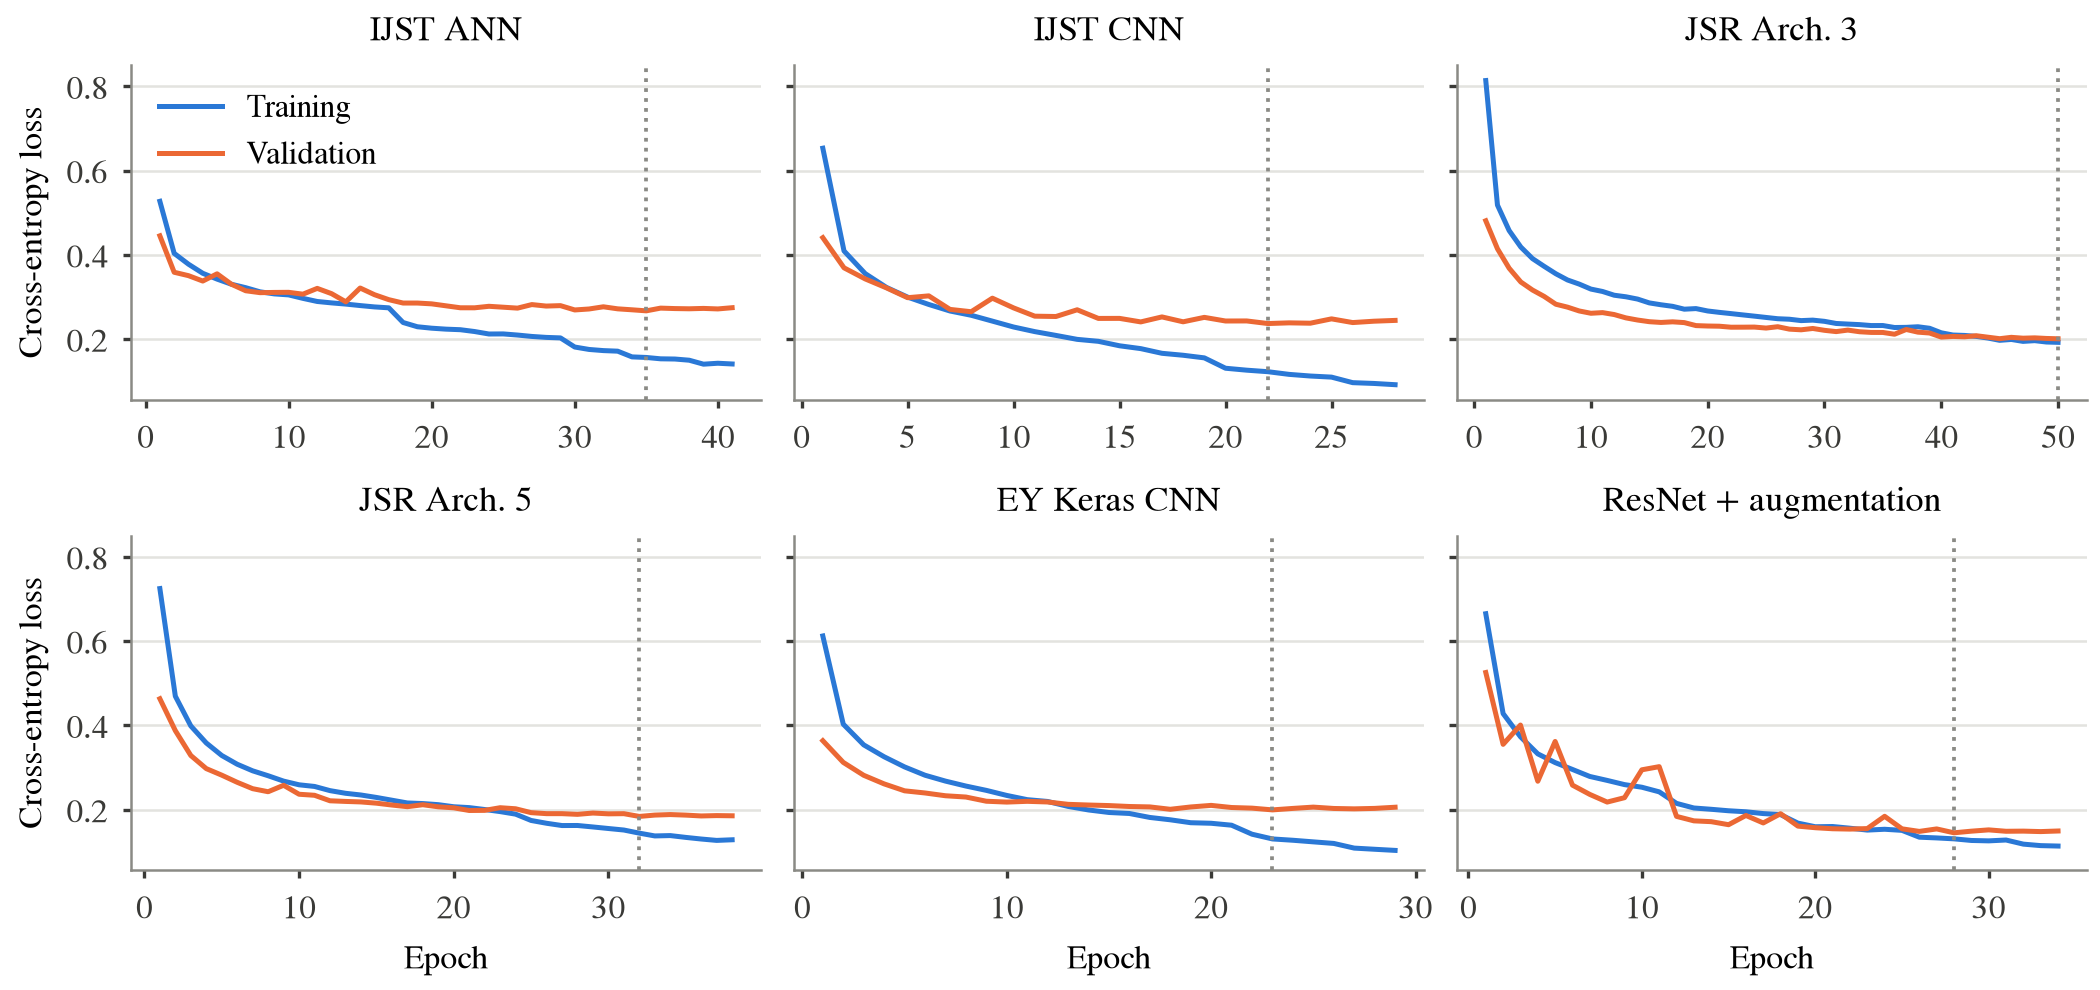
\includegraphics[width=\textwidth]{learning_curves.png}
\caption{Training loss (as trained, so with augmentation for the ResNet) and validation loss for the six networks trained on 48,000 images. The dotted line marks the epoch whose checkpoint was kept.}
\label{fig:curves}
\end{figure*}

\subsection{Published Models, ResNet and Ensemble}
Table~\ref{tab:neural} shows the networks trained on 48,000 images. On validation the ensemble scored highest (95.15\%), so it is the frozen final model. On the test set it reaches 94.19\% accuracy and 94.17\% macro-$F_1$, a 5.19-point improvement over the small CNN. The ResNet alone scores 94.32\%, slightly higher than the ensemble. This 0.13-point difference is smaller than single-seed variation, so we keep the validation-based choice rather than switch after seeing test scores. For every network, test accuracy is within about one point of validation accuracy, which indicates that the validation split was not overfitted.

\begin{table}[t]
\caption{Networks trained on 48,000 images: accuracy and macro-$F_1$ in \%, train--validation gap in points (test evaluated once)}
\label{tab:neural}
\centering
\small
\setlength{\tabcolsep}{4pt}
\begin{tabular}{@{}lrrrr@{}}
\toprule
Model & Val. & Test & $F_1$ & Gap \\
\midrule
\textbf{Ensemble (chosen)} & \textbf{95.15} & 94.19 & 94.17 & -- \\
ResNet + augmentation & 94.97 & \textbf{94.32} & \textbf{94.31} & \textbf{2.0} \\
Arch.~5~\cite{kadam2020cnn} & 93.76 & 92.74 & 92.72 & 3.4 \\
Keras CNN~\cite{edwards2019fashion} & 93.07 & 92.75 & 92.71 & 4.8 \\
Arch.~3~\cite{kadam2020cnn} & 92.87 & 91.90 & 91.90 & 2.8 \\
IJST CNN~\cite{sumera2022cnn} & 91.84 & 91.35 & 91.39 & 4.4 \\
ANN~\cite{sumera2022cnn} & 91.00 & 90.01 & 89.99 & 4.5 \\
\midrule
Small CNN (12,000 imgs) & 89.93 & 89.00 & 88.85 & -- \\
\bottomrule
\end{tabular}
\end{table}

\begin{figure}[t]
\centering
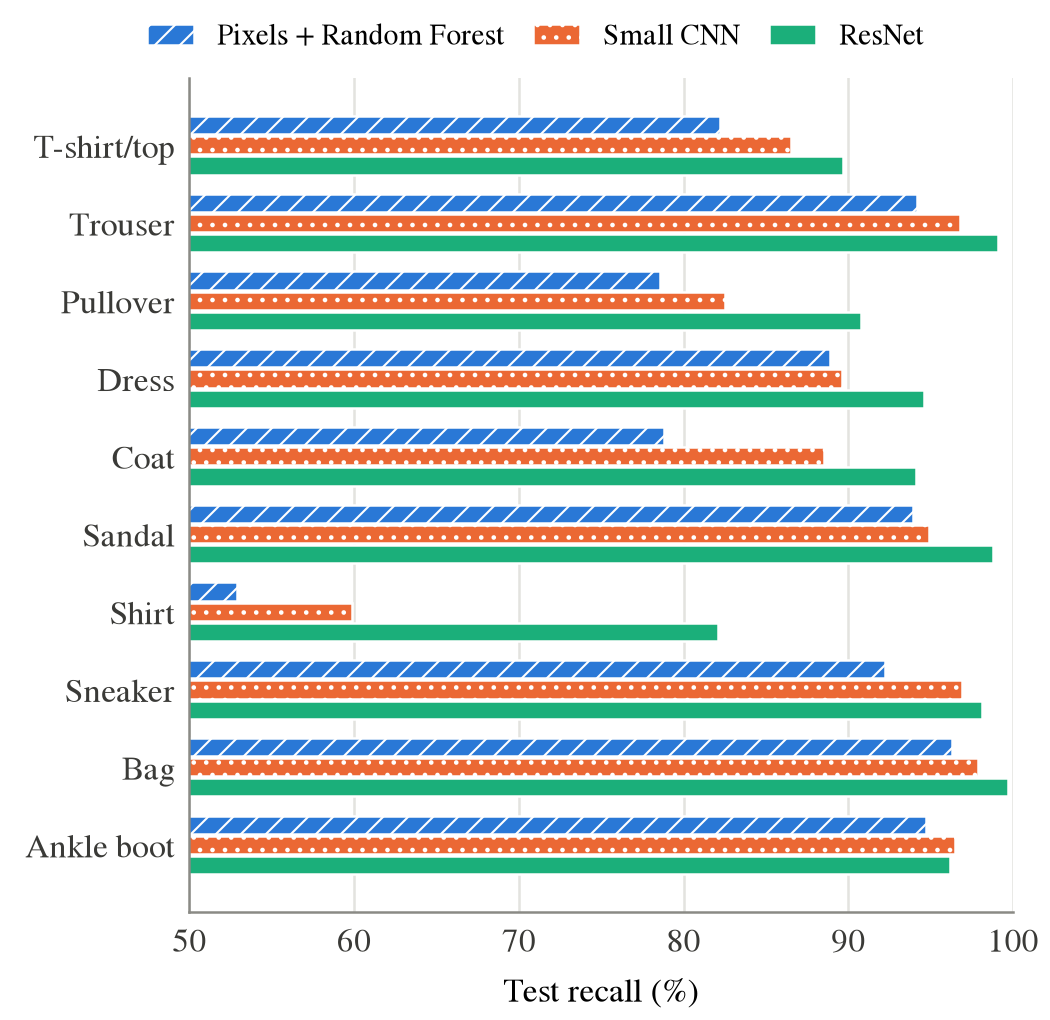
\includegraphics[width=\columnwidth]{per_class_recall.png}
\caption{Per-class test recall of the best classical model, the small CNN and the ResNet. Shirt recall rises from 52.9\% to 82.1\%.}
\label{fig:recall}
\end{figure}

Fig.~\ref{fig:curves} shows the learning curves. For the paper models without augmentation, training loss keeps falling after validation loss levels off. Early stopping catches this point, and the Keras CNN, with the largest dense layer, has the largest gap (4.8 points). The ResNet's training loss stays close to its validation loss throughout because augmentation makes the training task harder. The JSR Architecture~3 reached its best validation loss in the final allowed epoch, so it was still improving slowly and was not overfitting.

\subsection{Comparison with Reported Results}
Table~\ref{tab:reported} compares our reimplementations with the accuracies reported by the original studies. Agreement is within about two points. The remaining differences are expected: the originals trained on all 60,000 images, used fixed epoch budgets or other optimizers, and did not always state how the reported epoch was chosen. Our numbers come from 48,000 training images, a separate validation split and a single test evaluation.

\begin{table}[t]
\caption{Reimplemented models versus originally reported test accuracy}
\label{tab:reported}
\centering
\small
\begin{tabular}{@{}lrr@{}}
\toprule
Model & Reported (\%) & Ours (\%) \\
\midrule
ANN (Adam)~\cite{sumera2022cnn} & 88.0 & 90.01 \\
IJST CNN (Adam)~\cite{sumera2022cnn} & 91.0 & 91.35 \\
Arch.~3~\cite{kadam2020cnn} & 93.56 & 91.90 \\
Arch.~5 (Adam)~\cite{kadam2020cnn} & 93.56 & 92.74 \\
Keras CNN~\cite{edwards2019fashion} & 92.87 & 92.75 \\
\bottomrule
\end{tabular}
\end{table}

\section{Error Analysis}
Fig.~\ref{fig:recall} shows per-class test recall for the strongest model of each stage. Trousers, bags, sandals, sneakers and ankle boots are recognised reliably by all three models. Shirt is the hardest class throughout: its recall is 52.9\% for Random Forest, 59.9\% for the small CNN and 82.1\% for the ResNet. The small CNN's most frequent errors are all between upper-body garments: Shirt$\to$T-shirt/top (148 test images), Shirt$\to$Coat (127), Pullover$\to$Coat (111) and Shirt$\to$Pullover (83). These garments differ mainly in collars, buttons and sleeve length, details that are barely visible at $28\times28$ resolution. Edwards and Yen~\cite{edwards2019fashion} found the same pattern. The ResNet improves every upper-body class, with Coat rising from 88.5\% to 94.1\% and Pullover from 82.5\% to 90.8\%. Its gains come mostly from these confusable categories rather than from classes that were already easy.

\section{Deployment}
A Gradio~\cite{abid2019gradio} web application serves the ResNet on the local machine. An uploaded image goes through a fixed preprocessing contract. EXIF orientation is applied, the image is converted to grayscale, and images with a light background are inverted. The image is then resized bilinearly with its aspect ratio preserved and padded with black to $28\times28$. Native Fashion-MNIST images pass through unchanged. The interface shows the predicted category, all ten softmax scores and the exact $28\times28$ input given to the model.

The deployed predictor reuses this preprocessing code unchanged. It verifies the ResNet weights against a stored SHA-256 hash before loading them, and falls back to the small CNN if the ResNet is absent. The project is packaged with locked dependencies and a Docker Compose setup. A test suite checks the preprocessing contract, the architectures, the single-use test guards and the integrity of the frozen results.

\section{Limitations and Future Work}
Each network was trained with a single seed, so differences below about 0.5 points, including the ensemble--ResNet gap, are not statistically meaningful. The study uses $28\times28$ grayscale thumbnails, so its accuracy does not transfer directly to real product photographs with backgrounds, models, shadows or several items. Softmax scores are not calibrated probabilities. Future work includes multi-seed training with confidence intervals for the networks, wider residual networks~\cite{zhong2017random}, test-time augmentation, and evaluation on real catalogue photographs to measure how well the upload preprocessing generalises.

\section{Conclusion}
We compared classical classifiers, a small CNN, five networks from published studies and a residual network on Fashion-MNIST under a single protocol, with one test evaluation per frozen choice. Under a 12,000-image budget, the small CNN beats the best classical model, Random Forest on pixels, by 3.73 points. With 48,000 training images, batch normalisation, residual connections and random-erasing augmentation, the ResNet reaches 94.32\% test accuracy with the smallest train--validation gap. The validation-chosen ensemble reaches 94.19\%. Most of the remaining errors fall on shirts, whose details are barely visible at this resolution. The ResNet now powers the project's web demo.

\section*{Acknowledgment}
The authors thank their faculty guides, Shobhit Johri and Gourab Rajak, for their guidance throughout this project.

\begin{thebibliography}{00}
\bibitem{xiao2017fashion} H. Xiao, K. Rasul, and R. Vollgraf, ``Fashion-MNIST: A novel image dataset for benchmarking machine learning algorithms,'' arXiv:1708.07747, 2017.
\bibitem{sumera2022cnn} Sumera, R. Sirisha, N. Anjum, and K. Vaidehi, ``Implementation of CNN and ANN for Fashion-MNIST-dataset using different optimizers,'' \textit{Indian J. Sci. Technol.}, vol. 15, no. 47, pp. 2639--2645, 2022, doi: 10.17485/IJST/v15i47.1821.
\bibitem{kadam2020cnn} S. S. Kadam, A. C. Adamuthe, and A. B. Patil, ``CNN model for image classification on MNIST and Fashion-MNIST dataset,'' \textit{J. Sci. Res.}, vol. 64, no. 2, pp. 374--384, 2020, doi: 10.37398/JSR.2020.640251.
\bibitem{edwards2019fashion} C. Edwards and A. Yen, ``Fashion-MNIST,'' ECE 471 Final Project Report, Dept. Elect. Eng. Comput. Sci., Univ. of Tennessee, Knoxville, TN, USA, 2019. [Online]. Available: \url{https://cnedwards.com/files/Edwards_Yen_Final_Project.pdf}
\bibitem{bhatnagar2017classification} S. Bhatnagar, D. Ghosal, and M. H. Kolekar, ``Classification of fashion article images using convolutional neural networks,'' in \textit{Proc. 4th Int. Conf. Image Inf. Process. (ICIIP)}, 2017, pp. 1--6.
\bibitem{zhong2017random} Z. Zhong, L. Zheng, G. Kang, S. Li, and Y. Yang, ``Random erasing data augmentation,'' arXiv:1708.04896, 2017.
\bibitem{he2016deep} K. He, X. Zhang, S. Ren, and J. Sun, ``Deep residual learning for image recognition,'' in \textit{Proc. IEEE Conf. Comput. Vis. Pattern Recognit. (CVPR)}, 2016, pp. 770--778.
\bibitem{ioffe2015batch} S. Ioffe and C. Szegedy, ``Batch normalization: Accelerating deep network training by reducing internal covariate shift,'' in \textit{Proc. Int. Conf. Mach. Learn. (ICML)}, 2015, pp. 448--456.
\bibitem{dalal2005hog} N. Dalal and B. Triggs, ``Histograms of oriented gradients for human detection,'' in \textit{Proc. IEEE Conf. Comput. Vis. Pattern Recognit. (CVPR)}, 2005, pp. 886--893.
\bibitem{breiman2001random} L. Breiman, ``Random forests,'' \textit{Mach. Learn.}, vol. 45, no. 1, pp. 5--32, 2001.
\bibitem{cortes1995support} C. Cortes and V. Vapnik, ``Support-vector networks,'' \textit{Mach. Learn.}, vol. 20, no. 3, pp. 273--297, 1995.
\bibitem{kingma2015adam} D. P. Kingma and J. Ba, ``Adam: A method for stochastic optimization,'' in \textit{Proc. Int. Conf. Learn. Represent. (ICLR)}, 2015.
\bibitem{pedregosa2011scikit} F. Pedregosa \textit{et al.}, ``Scikit-learn: Machine learning in Python,'' \textit{J. Mach. Learn. Res.}, vol. 12, pp. 2825--2830, 2011.
\bibitem{paszke2019pytorch} A. Paszke \textit{et al.}, ``PyTorch: An imperative style, high-performance deep learning library,'' in \textit{Adv. Neural Inf. Process. Syst. (NeurIPS)}, 2019, pp. 8024--8035.
\bibitem{efron1993bootstrap} B. Efron and R. J. Tibshirani, \textit{An Introduction to the Bootstrap}. New York, NY, USA: Chapman \& Hall, 1993.
\bibitem{abid2019gradio} A. Abid, A. Abdalla, A. Abid, D. Khan, A. Alfozan, and J. Zou, ``Gradio: Hassle-free sharing and testing of ML models in the wild,'' arXiv:1906.02569, 2019.
\end{thebibliography}

\end{document}
